%%%%%%%%%%%%%%%%%%%%%%%%%%%%%%%%%%%%%%%%
% WHCS Senior design conference paper
%   Written at UCF in 2015 
%   Typeset by Grant Hernandez
%   For authors, see the title page
%%%%%%%%%%%%%%%%%%%%%%%%%%%%%%%%%%%%%%%%

% What type of document are we building here
\ifdefined\enabledraft
  \documentclass[draft,twocolumn,letterpaper,10pt]{IEEEtran}
\else
  \ifdefined\enablefinal
    \documentclass[final,twocolumn,letterpaper,10pt]{IEEEtran}
  \else
    \documentclass[twocolumn,letterpaper,10pt]{IEEEtran}
  \fi
\fi

% not sure if should prefer IEEE default
\usepackage[tmargin=1.125in, bmargin=1.125in, lmargin=0.85in, rmargin=0.85in]{geometry}

%%%%%%%%%%%%%%%%%%%%%%%%%%%%%%%%%%%%%%%%
% Packages
%%%%%%%%%%%%%%%%%%%%%%%%%%%%%%%%%%%%%%%%

% Common color names
\usepackage[usenames,svgnames]{xcolor}
% For \textsubscript
\usepackage{fixltx2e}
% For meeting senior design specifications
%\usepackage{parskip}
% For easy importing of documents
\usepackage{import}
% For the checkbox and other math symbols
\usepackage{amsmath}
\usepackage{amssymb}
% Advanced captions
\usepackage{caption}
\usepackage{wrapfig}
% TODO tracking
\usepackage[obeyFinal,colorinlistoftodos,prependcaption,textsize=tiny]{todonotes}
% Fancy section headings
%\usepackage{titlesec}
% TikZ madness
\usepackage{tikz}
\usetikzlibrary{shapes.misc}
% Filler text
\usepackage{lipsum}
% Wrapping text around figures
\usepackage{wrapfig}
% For pretty code listings
\usepackage{listings}
% Keep floats in check with [H]
\usepackage{float}
% For including raw PDFs
\usepackage{pdfpages}
% Fancy if statements
\usepackage{ifthen}
\usepackage{array}
% for \affil
\usepackage{authblk}
%\usepackage{booktabs,adjustbox}
%\usepackage{supertabular}

%%%%%%%%%%%%%%%%%%%%%%%%%%%%%%%%%%%%%
% Hyperref should be last
%%%%%%%%%%%%%%%%%%%%%%%%%%%%%%%%%%%%%
% Document jumping and linkage
% NEVER use draft mode for hyperref
\ifdefined\enabledraft
  \usepackage[draft=false]{hyperref}
\else
  \usepackage{hyperref}
\fi

% Probably not needed for now
%\usepackage{setspace}
%\usepackage{fancyhdr}
%\usepackage{wrapfig}
%\usepackage[binary-units]{siunitx}

%%%%%%%%%%%%%%%%%%%%%%%%%%%%%%%%%%%%%%%%
% Color Palette
%%%%%%%%%%%%%%%%%%%%%%%%%%%%%%%%%%%%%%%%
% Code Colors
\definecolor{CommentGreen}{rgb}{0,0.6,0}
\definecolor{numbering}{gray}{0.5}
\definecolor{keywordc}{rgb}{.63,0,.42}

% Title page
\definecolor{whcs-accent}{HTML}{A66AFF}
\definecolor{whcs-accent-dark}{HTML}{6600FF}
\definecolor{whcs-muted}{HTML}{555555}

%%%%%%%%%%%%%%%%%%%%%%%%%%%%%%%%%%%%%%%%
% LaTeX Configuration & Macros
%%%%%%%%%%%%%%%%%%%%%%%%%%%%%%%%%%%%%%%%

% Keep our graphics nice and neat
\graphicspath{{img/}}

% Customize hyperref
\urlstyle{same} % remove monospaced links
\ifdefined\printable
\hypersetup{pdfnewwindow=true, % prevent the user from leaving the paper
hidelinks,
% PDF Meta
pdftitle={Wireless Home Control System - UCF Senior Design I},
pdfsubject={University of Central Florida Senior Design 2015},
pdfauthor={Grant Hernandez},
}
\else
\hypersetup{pdfnewwindow=true, % prevent the user from leaving the paper
colorlinks,
linkcolor={whcs-accent-dark},
citecolor={blue!50!black},
urlcolor={blue!80!black},
% PDF Meta
pdftitle={Wireless Home Control System - UCF Senior Design I},
pdfsubject={University of Central Florida Senior Design 2015},
pdfauthor={Grant Hernandez},
}
\fi

% Customize autoref names
% See page 16 of hyperref manual
\renewcommand\sectionautorefname{Section}
\renewcommand\subsubsectionautorefname{Section}
\renewcommand\subsectionautorefname{Section}
\renewcommand\paragraphautorefname{Section}

% Custom figure macro for quick and easy changes across the document
%   \ucffig
%     Param 1: label
%     Param 2: figure content
%     Param 3: caption
\newcommand{\ucffig}[3]{
\begin{figure}[h]
\centering
\makebox[\linewidth][c]{
#2
}
\caption{#3}
\label{#1}
\end{figure}
}

\newcommand{\ucfgfx}[4][scale=1.0]{
\ucffig{#2}{\includegraphics[#1]{#3}}{#4}
}

% TBW macro
\newcommand{\tbw}{\emph{This section is in the process of being written.}}

% Section Heading Customization
\ifdefined\printable
\else
  \ifdefined\enabledraft
  \else
    %\newcommand\titlebar{%
    %  \input{section-heading.tex}
    %}
    %\titleformat{\section}{\bfseries\Large}{\color{white}\titlebar}{0.1cm}{}
    \newcommand\titlebar\relax
  \fi
\fi

% Disable images on draft mode
\ifdefined\enabledraft
  \renewcommand{\includegraphics}[2][]{}
  \renewcommand{\includepdf}[2][]{}
\else
\fi

\renewcommand*{\thesection}{\arabic{section}}

% A custom listing format
\lstdefinestyle{code}{%
  basicstyle=\ttfamily\small,
  language=php,
  numbers=left,
  numberstyle=\footnotesize\color{numbering},
  fontadjust=true,
  basewidth=0.5em,
  % flexiblecolumns=true,
  keywordstyle={\bfseries\color{magenta}},
  commentstyle=\color{CommentGreen},
  stringstyle=\color{red},
  showstringspaces=false,
  tabsize=4,
  %xleftmargin=\MaxSizeOfLineNumbers
}

%=%=%=%=%=%=%=%=%=%=%=%=%=%=%=%=%=%=%=%
% BEGIN DOCUMENT
%=%=%=%=%=%=%=%=%=%=%=%=%=%=%=%=%=%=%=%
\begin{document}
\pagenumbering{gobble}

% We want this depth for our TOC
\setcounter{secnumdepth}{3}
\setcounter{tocdepth}{4}

%%%%%%%%%%%%%%%%%%%%%%%%%%%%%%%%%%%%55
% Title
%%%%%%%%%%%%%%%%%%%%%%%%%%%%%%%%%%%%55
\begin{center}
\huge Wireless Home Control System
\vspace{0.5cm}

\large Grant Hernandez, Jimmy Campbell\\ and Joseph Love
\vspace{0.5cm}

\large Dept. of Electrical Engineering and Computer Science, University of Central Florida, Orlando, Florida, 32816-2450  
\vspace{0.5cm}
\end{center}

\begin{abstract}
The presence of wireless technologies and proliferation of mobile controlled devices have inspired a push toward consumer based home automation systems. Wireless Home Control System is a home automation framework designed to compete with popular solutions in the domain. The system features peripheral control modules capable of interacting with lights, outlets, doors, and sensors. All control modules communicate with a central hub that is paired with a mobile device to provide total control to the user. We describe the hardware and software necessary to conceive this system.
\end{abstract}

\begin{IEEEkeywords}
bluetooth, Home automation, mobile, scalable platform, sensors, power control, wireless.
\end{IEEEkeywords}

%%%%%%%%%%%%%%%%%%%%%%%%%%%%%%%%%%%%%%%%%%%%%%%%55
% Intro
%%%%%%%%%%%%%%%%%%%%%%%%%%%%%%%%%%%%%%%%%%%%%%%%55
\section{Introduction}
Wireless Home Control System (WHCS) is a solution for any homeowner to
be able to remotely control core appliances of their home. WHCS
allows the user to control lights, outlets, doors, and sensors around their
home. The system{}'s design philosophy emphasizes ease of use, affordability,
and effectiveness. An Android phone application developed for WHCS allows
users to monitor the state of the installed components and activate them
remotely. A central base station equipped with a touch{}-enabled LCD is
present, allowing the users to interact with the system without the need of a
phone. Peripheral control modules may be installed into targeted
appliances such as lights, outlets, and doors for WHCS to control. As shown in \autoref{fig:whcs-overview}, the
phone, base station, and peripheral control modules constitute WHCS.

The implementation of such a system required research in a myriad of fields to
produce a full{}-fledged product. A well designed Android application is the key to
creating a positive first impression of WHCS. Thus, care was taken to
conform to the design philosophies of the Android ecosystem. The alternative
interface offered for WHCS is the base station{}'s display. Communication
devices form the foundation for the wireless aspect of WHCS, thus an
investigation into the advantages of different communication modules was
required to realize the system. A network protocol has been developed
and implemented in order to form a unified system from the independent modules.
The activation of appliances around the home requires high voltage control, so
methodologies for properly harnessing the power provided by homes were researched.
To extend upon harnessing the home{}'s power, our individual
control modules and base station{}'s logic level voltages (5V) depend upon the
creation of an efficient way to step down the high voltage supplied from the
home.

\ucfgfx[width=\linewidth]{fig:whcs-overview}{a21expected2pages-img001.png}{WHCS System Overview}

% Base Station
\section{Base Station}
The heart of WHCS resides with the base station (BS). When users think of WHCS, they
will think of the base station as it is the most visible hardware component of the system.
Powered by an AVR Atmega32-A, the base station is responsible for managing, collecting, and displaying
information from all of the control modules. If the BS were to fail, WHCS
would cease to function.

\subsection{Subsystems}
The base station has the hardest job in the entire WHCS architecture. It has to
juggle a lot of data with limited memory and processing speed. Packets need to be
processed and queued to keep the pipeline flowing smoothly. The radio,
bluetooth, LCD, and touchpanel need to be managed and updated in real time.

\subsubsection{NRF24L01+}
The NRF radio is directly connected to the Atmega32-A microcontroller
through the SPI bus. The radio job is to constantly listen for new
packets from the control modules and sending responses in turn. 
Also, when a command such as "open door" needs to be sent, the radio
switches to transmit mode in order to send the corresponding packet.

In WHCS' architecture, the main loop of the base station is not
interacting directly with the radio. This is due to the abstraction we
built around the low-level radio driver. All driver specific functions are
be wrapped in to a fa\c{c}ade pattern, network library. This allows WHCS
to swap out the underlying network hardware for another, similar radio if
needed.  Due to this
radio being the most critical for WHCS, it needed to have the most attention to
detail when constructing the layout and software design. In order to meet these
tight constraints, we chose the popular and well support RF24 library. This
library is used by many other projects and has a proven track record.
Additionally, members already had experience working with the API, therefore
the learning curve was quite low.

\subsubsection{HC-05}
The HC-05 Bluetooth module is quite simple in its operations. Data is sent over
a two line serial bus and if there is an active connection to a bluetooth
enabled device, it is easily able to receive the data and handle it. In
this case the device on the other end is expected to be a phone, but not
limited to one. As long as the device on the other end of the Bluetooth link
follows the WHCS Bluetooth application protocol, then WHCS is able to
receive commands from arbitrary devices. In order to pass messages across this
medium, a binary protocol has been developed. A simple
diagram showing a very high level interaction of a Bluetooth device with the base
station is for reference in \autoref{fig:android-comm}. Once again
this underlying protocol is abstracted away from the underlying
hardware. For example, if the HC-05 were to fail to meet WHCS' strict
requirements, then we would have to switch it for the next best unit - the
RN-41. If we wrote the underlying driver to be the ``top level'' layer that the
base station interacts with, then a large amount of code and possibly
architecture would have to be swapped out to meet the needs of another hardware
device.

In regards to the application level protocol for WHCS, there is a
well defined, easy way, for the Bluetooth library to gather information from
WHCS' state. This is handled on the top-level flow of the base station by
gluing together two different libraries without them knowing about each other.
This is a good approach because it decouples the two modules from each
other, making their individual implementations separate. Two tightly coupled
modules may start to take on the appearance of a ``ball of mud.'' A connected
phone is able to accomplish any task that manually interacting with the
LCD can handle. This includes controlling the function of individual
modules and querying their current state. The BT connection tries to avoid
generating too many packets over the NRF radio in response to user events.
Instead it merely lookups the cached state from the base station's memory.
This is faster and the round trip time is quick. Also, if a
bluetooth packet requires a radio packet to be generated, this
interaction is asynchronously tracked until the request has been
fulfilled.

\subsubsection{LCD}
In what could be considered the ``face of WHCS'', the LCD module is
situated directly over the Atmega32-A. It has the tough job of accurately
and quickly conveying any desired information about the state of WHCS' control
modules. This was no simple task as not only does it have to display, but with
an attached touchpanel, it has to react to user touches. What functionality is
exported to the LCD is only limited by the underlying processor speed and the
UI library. The high level design of the WHCS LCD only had to worry about
what the end goals are for its usage. An example of this abstraction may be
viewed in \autoref{fig:lcd-soft-hier}.

\ucfgfx[width=\linewidth]{fig:lcd-soft-hier}{lcd-soft-hier}{the level of abstractions for the LCD
subsystem}

As the state of the WHCS network changes, the base station fires
off redraw events in order to keep the LCD up-to-date. These redraws sync
the internal state of WHCS with the user viewable interface. The physical
connections to the LCD consist of data signaling and an 8-bit wide
parallel data bus. There is an optional reset pin that WHCS uses for
emergency resets and debugging. The high level interface with the LCD works
directly with the high-level UI library and if necessary the underlying
graphics library. The base station should never use the direct driver interface
as this is subject to change due to hardware revision. 
In addition, a subtle feature that WHCS may choose to implement would be
dynamic power saving through screen dimming. Although we assume the base
station has wall power at all times, there may come a time where the
system may migrate over to a lower wattage current source, such as power
stealing from an HVAC unit. In this case, the system would most certainly have
to be power efficient. Despite not needing to worry about power, this function
would be simple to implement as only one microcontroller pin is required to
control the screen brightness.

\subsubsection{Touchpanel}
In order to provide a way for an end user to be able to control WHCS from the
LCD unit, there is a requirement to poll for touch events.
This subsystem can be considered a part of the LCD, but the driver is independent
from the graphics and ILI9431 (LCD) drivers. These events are be dispatched
to the appropriate UI element  based on the X and Y position of the touch
event. There is an optional Z ``position'' which represents the pressure,
which is used to gather more fine grained information
about the touch itself. One of the unfortunate properties of the touchpanel is
that it must be actively polled for new touches. This required that the ADC be
constantly providing conversions, which raises the dynamic power of the MCU.
This isn't a major concern as the base station is expected to have power from the wall
most of the time.

The extent of the touchpanel interaction occurs from a \texttt{getTouch()}
method. This method returns the latest touch event, if any. The base
station has full control over where this touch event is dispatched to.
Depending on the LCD scene (i.e main menu, boot screen), this event is be
handled in different ways.

\subsection{Software Architecture}
The code for the base station is the most complicated in WHCS. It has to manage
three separate devices simulatenously and be able to service each one in a
timely manner. The LCD, NRF radio, and Bluetooth module are all being
controlled and commanded by one ATMega32-A chip. There isn't much room for busy
waiting or any expensive operations as everything has to be running as fast as
possible. Given this, the BS is the least point of failure for the WHCS. This
complicated main loop, including early initialization, may be seen in
\autoref{fig:base-station-flow}.

\ucfgfx[width=0.8\linewidth]{fig:base-station-flow}{base-station-flow}{The high level software flow for the base station}

Starting from reset, the base station first loads any saved settings from the
EEPROM (saved control modules, behavior settings, LCD settings, etc.), then it
brings up all of the main classes (radio, LCD, Bluetooth, and UART).
Each subsystem has a unique sequence of ``commands'' with parameters that are
required to configure the device. The NRF radio has to have its power, channel,
payload length, and other parameters set before usage. Once these basic
options are set, any further configuration is done at run time. This includes
switching from listening to transmitting mode and enabling or disabling the
automatic acknowledgement feature. The built-in Atmel UART only needs to know
the baud rate at which data will be sent and received. 
The LCD happens to have the most extensive initialization sequence due to
required screen configuration, gamma settings, pixel order and other more
archaic options.

Once all of the subsystems are brought up correctly, the BS begins the main loop.
Radio events, Bluetooth events, and LCD state are all processed as
required. For both the Bluetooth and radio, new packets are checked
and serviced as needed. From these packets, internal state would updated and any
response packets would be generated and sent. Internally, WHCS has an
internal event queue with different event types. These events are processed
and any responses are generated, if any. These responses could include a
confirmation packet over the NRF radio, or a status update through Bluetooth.
The base station may also initialize actions despite not receiving events.
These could be triggered from timers firing.

All of the above tasks are executing in the same way as single core CPU
would: in pseudo-parallel. The faster the whole system runs, the better the
appearance of everything executing at once.

\subsection{Control Module Abstraction}
For WHCS to function smoothly and scale well, a neat and abstracted interface
must be defined to accept \emph{any} type of control module. New control module
types should be easily added to the system without affecting older types and
there should be a set of generic data structures for managing and storing
information on modules. These structures must be carefully defined to wrap more
specific control module packets in all of the shared metadata. Think of it like
a hierarchy where all of the common attributes and actions shared by control
modules have packets that can be sent to any module. Whereas the more specific
packets (get temperature, engage door, etc.) would be wrapped up in the generic
ones (essentially a derived object from the generic control module.) This can
be visualized in \autoref{fig:ctrl-mod-hierarchy}. The
details of a network structure that would enable this clean interface is
further described in \autoref{sec:network-library}.

\ucfgfx[width=\linewidth]{fig:ctrl-mod-hierarchy}{control-module-hierarchy}{showing the control
module hierarchy for WHCS}

Beyond sending packets, the base station must accurately record and update
state for all of the control modules. Depending on the control module,
additional state is stored. Each control module has its own state machine that
controls its function in relation to the base station.

\subsection{Schematic Breakdown}
To tie the whole design of the base station together, the schematic, created in
KiCad is broken down below.

In \autoref{fig:bs-sch-crystal} we see a focused view of the Atmega32-A
microcontroller with an attached 16MHz crystal and power passives. The crystal
has two capacitors that are dependent on the target crystal. These are required
to get the correct oscillation for the external crystal. Also the AREF, VCC,
and AVCC lines of the MCU have decoupling capacitors. These are used to make
sure that the base station performs well under a large current spike. When
designing the board, these capacitors should be placed as close as possible to
the MCU to avoid a long high-current path through the ground plane. The
capacitor on the analog reference pin (AREF) is used to stabilize the reference
to make ADC conversions more accurate.

% Zoom in on the crystal setup and decoupling caps
\ucfgfx[trim=1in 5.0in 5.1in 0.5in,clip,width=\linewidth]
{fig:bs-sch-crystal}{base-station.pdf}{Base Station crystal and decoupling capacitors}

In \autoref{fig:bs-sch-lcd-header} we see the buses used to connect the LCD to the
MCU. This is the most pin heavy component and care must be taken not to mix up
any of the signal paths. All of the data control signals are connected to PORTD
of the MCU, the touchpanel signals to PORTA (ADC), and the 8-bit parallel data
bus completely uses PORTC. There are a few one off signals such as LITE which
is a PWM input to control the LCD's backlight brightness.

% Zoom on the LCD header
\ucfgfx[trim=4.2in 3.3in 2.5in 1.55in,clip,width=\linewidth]
{fig:bs-sch-lcd-header}{base-station.pdf}{Base Station LCD header to MCU}

In \autoref{fig:bs-sch-pwr-nrf} we see the 3.3V 3 terminal regulator converting the
5V VCC line down. Additionally, we see the external RESET pull-up resistor and
a manual reset push button. The left corner has the pinout for the NRF breakout
board we are using.

% Zoom on the power section and NRF
\ucfgfx[trim=5.9in 1.3in 1.2in 5.0in,clip,width=0.95\linewidth]
{fig:bs-sch-pwr-nrf}{base-station.pdf}{Base Station power schematic and NRF header}

In \autoref{fig:bs-sch-hc-05} we see the header for the HC-05. We examine this
further because of the unique electrical characteristics of the HC-05 module.
The module only accepts 3.3V power and logic. Our MCU is running at 5V,
which means we need a 5V to 3.3V logic shifter. To simply implement this, we
used a resistor voltage divider which provided the required logic level for
the TX pin. The RX pin does not need a shifter because 3.3V is still above the
$V_{IH}$ minimum for the MCU.

% Zoom on the HC-05
\ucfgfx[trim=1.0in 1.0in 7.5in 5.0in,clip,width=0.8\linewidth]
{fig:bs-sch-hc-05}{base-station.pdf}{Base Station HC-05 header}

Finally, in \autoref{fig:bs-sch-isp} we see the standard ICSP header that most
AVR line microcontrollers use. This pin array serves as a quick and easy
way to connect an external programmer to our base station while in the field.
In this schematic revision, this header can provide power directly to the 3.3V
regulator and MCU.

% Zoom on ISP header
\ucfgfx[trim=1.2in 3.8in 8.2in 4.0in,clip,width=0.6\linewidth]
{fig:bs-sch-isp}{base-station.pdf}{Base Station ISP header}

% Control Modules
\section{Control Modules}
What can be thought of as the ``arms of WHCS'', the control modules serve as
the main devices that seed the network with data. This data is specific to the
control module that is emitting it. The base station is more more complex than
an individual control module because it needs to be. The control modules should
be as lightweight as possible to save cost and keep power usage down. If the
control modules were too complex, then the entire cost of WHCS would increase
proportionally to the number of control modules.

\subsection{Software Flowchart}
The general flow for the control modules is much simpler than the base station
just due to the requirements of the system. There isn't as much that needs to
be done on each loop iteration. The only main module that the control module
needs to work with is the NRF radio. This can be seen in
\autoref{fig:ctrl-mod-soft-flow}. Due to the capabilities
for the NRF radio to provide an interrupt signal on the reception of a packet,
the control module actually has the ability to sleep when not doing anything.
Control modules should be as mobile as possible, which limits their overall
functionality and processing power. Without these limits, any battery attached
would quickly be drained.

\ucfgfx[width=\linewidth]{fig:ctrl-mod-soft-flow}{control-module-flow}{the high level
software flow for a generic control module}

\subsection{Electronic Strike}

\label{sec:electronic-strike}

WHCS features an electronic strike which allows control modules to lock and
unlock doors within the system. The electronic strike was chosen over an
electronic deadbolt because the strike can still be used with a normal door
knob. If the electronic strike ever fails during operation the door knob can be
unlocked and therefore bypass the strike system. This design principle gets rid
of safety hazards that could occur if the WHCS system lost power. The operating
mode for the electronic strike is normally open. This means the strike requires
power to be unlocked and is otherwise locked. As a result, power is saved
within the system which is beneficial because the electronic strike consumes
roughly 450 mA at 12V during operation.

\subsection{Sensor Data Collection}
The temperature sensor that we used for WHCS is the TMP36. The temperature
sensor is simple in design as it has only three pins that require connection.
The schematic shown in \autoref{fig:temp-sensor-connect} shows how the
temperature sensor is connected to the ATmega328 on the control modules. The
VOUT pin of the TMP36 outputs a voltage signal that varies based on the
temperature surrounding the component.  The voltage range is between 2.7 to 5.5
volts which is supplied through or logic level voltage lines. This sensor has a
rated temperature range of -40 to 125 degrees Celsius which is broad enough for
a household temperature sensor.

\ucfgfx[width=\linewidth]{fig:temp-sensor-connect}
{a683SensorCollectionexpected2pages-img001.png}{Temperature Sensor Connection Schematic}

\subsection{Light and Outlet Control}
The solution to controlling lights and outlets in WHCS is through an AC solid
state relay. The solid state relay that we use is capable of switching a load
of 120V AC up to 16A. The activation voltage is 1.2V and the activation current
is 15mA. The ratings of the chip allow the relay to be controlled directly from
the control module’s microcontroller GPIO pins. This solid state relay’s small
activation requirements provide low power operation capabilities as well as
design simplicity. \autoref{fig:wiring-sch-ssr} shows a schematic using this
solid state relay.

\ucfgfx[width=\linewidth]{fig:wiring-sch-ssr}{a684LightandOutletControl-img001.png}{
Wiring Schematic for Solid State Relay}

\subsection{Schematic Breakdown}
The control modules for WHCS have to be able to support communication via a
radio transceiver as well as interaction with their target endpoints.
\autoref{fig:ctrl-mod-sch} shows the schematic for the control modules that is be
implemented in WHCS. The full schematic is available for viewing in \autoref{apx:control-module-sch}. The main component of the schematic is the ATmega328.
Everything in the schematic is connected to the microcontroller in some way. In
the schematic three different VCC lines are shown. This is because the control
modules will have to access to a 3.3V line, a 5V line, and a 12V line. The
power board will supply these power lines to the control module. The 5V and
3.3V lines are necessary because they provide power to the logic chips like the
microcontroller and the radio transceiver. The 12V line is necessary solely for
the electronic strike that we have chosen.

\ucfgfx[width=\linewidth]{fig:ctrl-mod-sch}{a686SchematicBreakdownExpected2pages-img001.png}
{WHCS Control Module Schematic}

%%%%%%%%%%%%%%%%%%%%%%%%%%%%%%%%%%%%%%%%%%%%%%
% Android Application
%%%%%%%%%%%%%%%%%%%%%%%%%%%%%%%%%%%%%%%%%%%%%%
\section{Android Application}
For most WHCS users the mobile application
will be the only physical interaction they have with the application. When we
set out for development we wanted to make an easy to use application that would
attract users to stick with our system.  Operability and usability were
emphasized in our design process. We wanted an appealing U.I. without
complexity, after all we are targeting a simple solution to home automation.

\subsection{Bluetooth Software Design}
Bluetooth is the technology allowing the Android application to communicate
with the base station. The first step of the Bluetooth lifecycle is to ensure
that Bluetooth is enabled. When it has confirmed that Bluetooth is on, the
application will the user to connect to a base station. When connecting to a
device there are two possibilities for connection, paired devices and
non-paired devices. The application will first show the user all devices that
their phone has paired with previously such as the base station.  If the base
station does not show up in the paired devices list, the user will be able to
search for active Bluetooth devices and select the base station. At the end of
this start up cycle the WHCS application will have an active Bluetooth
connection with the base station that can be used for full duplex
communication. A socket can be opened within the android application for
communication between the two Bluetooth devices.

Once a \texttt{BluetoothSocket} has
been opened on the Android device the application can begin communicating with
the base station. We use a custom communication protocol between the Android
device and base station to ensure proper interaction. This protocol allows the
Android application to give commands to the base station such as inquire about
the state of the control modules or to toggle state within the system. Whenever
the Android application wants to send a message to the base station the
software creates a packet with a certain structure. The packet contains a byte
for letting the base station know that a command is being given, the command
itself, any variables for the command, and then a byte for finishing the
command. The base station receives one byte at a time due to the serial nature
of Bluetooth communication but it is able to parse the packets it receives in
order to figure out what action the application is trying to perform. \autoref{fig:android-comm} shows a visual representation of the communication between the application and
the base station.

\ucfgfx[width=\linewidth]{fig:android-comm}{a55-img005.png}{Visual of Communication Between
Android Device and Base Station}

\subsection{Speech Recognition}
The Android application for WHCS offers speech activation capabilities. These
are on top of GUI activation capabilities. The speech activation sequence
begins with the press of a button to start the speech recognition. The user is
prompted with a microphone and can then give his command. The commands are
formatted similarly to “light one on.” When the user gives commands using the
speech method, a notification is given indicating the success of interpreting
the speech into a known command. If the user’s speech does not match a known
command, the speech is shown back to the user to show what went wrong. The
following flowchart in \autoref{fig:android-speech} displays the sequence of events happening when
a user performs speech activation.

\ucfgfx[width=\linewidth]{fig:android-speech}{a55-img003.png}{Android app speech activation
chart}

%%%%%%%%%%%%%%%%%%%%%%%%%%%%%%%%%%%%%%%%%%%%%%
% Power Hardware
%%%%%%%%%%%%%%%%%%%%%%%%%%%%%%%%%%%%%%%%%%%%%%
\section{Power Hardware}
\label{sec:power-hw}
In order to power our system we stepped down the 120VAC found in homes to the
voltages that our system requires. For our system we need a 12V, 5V, and 3.3V
lines. To provide these lines we used a traditional full bridge rectifier
design using a 60 Hz 120:14 transformer to convert our AC voltage down to
19.8VDC. We considered using a switched mode power supply, yet based on the
increase of complexity of SMPS designs we decided that we would not have enough
time to incorporate this type of design for our AC to DC power step down. After
having stepped down the power we used TI WEBENCH to convert the 19.8VDC to 12V,
5V, and 3.3V lines. Each line was made using switching regulators in order to
have maximum efficiency.

%\autoref{fig:power-sch} below shows the basic flow of our power design. 120VAC
%is fed into the board. This voltage is stepped down by the transformer then
%rectified by the rectifier. The resulting 20VDC is fed into both the 5V and 12V
%switching regulator. The 3.3V switching regulator draws its voltage from the
%output of the 5V switching regulator.

%\ucfgfx[width=\linewidth]{fig:power-sch}{Schematicbreakdown-img001.png}{Power hardware schematic breakdown}

\subsection{Power Consumption}
\label{sec:power-consumption}
Power consumption wasn{}'t a top priority in our design. While it is important
not to be incredibly wasteful to the point that it becomes a problem, power was
not something that we decided we wanted to be competitive on. Had we wanted to
be more competitive with power, we would have taken a lot more into account and
made different design decisions. For example with the microcontrollers we would
have looked more carefully into the amount of current that they drew to help us
weigh our decisions. MSP430 boards for example would have been attractive
because of the low amounts of current that they draw. With that said we made
all of our decisions based on their performance and ease of integration. We
merely needed to know how much current our system drew to properly design of
our switching regulators as well as choose our transformer.

The \autoref{tbl:powerconsump} and \autoref{tbl:powerconsump2} were used in making our design decisions.

\ucfgfx[width=0.8\linewidth]{tbl:powerconsump}{Powerconsump-img001.png}{shows the current requirements of each device in our system.}

\ucfgfx[width=0.54\linewidth]{tbl:powerconsump2}{Powerconsump-img002.png}{shows what the max current for each line in our system at any point in time.}

\subsection{Transformer and Capacitor Choice}
To choose the transformer we needed to take into account the apparent power
rating as well as the winding ratio. Given that the highest voltage output
needed for our design was 12VDC we decided on a 120:14 winding ratio. This gave
us about 20VDC to be stepped down by our switching regulators. To choose the
apparent power rating we had to consider the current draw. From
\autoref{tbl:powerconsump2} we find that the max current the system would could ever
draw would be below 725 mA. The apparent power rating can be calculated by
I*Vrms. Given the information of our system we required an apparent power
rating of at least .725*14 = 11. The transformer we chose had an apparent power
rating of 20. 

We chose our capacitor using the equation $V_r = \frac{I}{2*f*C}$ for an approximation
of the expected ripple (Millman-Halkias, pg. 112-114). Using a capacitor of
$4700\mu~F$ gives us a ripple of .887V (for most applications our current draw will
be below 500 mA).

% Conclusion
\section{Conclusion}
Through extensive research, design, and implementation WHCS was realized to
meet all requirements set. The Android application was architected successfully
for simplistic interaction. All use cases were implemented in order to provide
the optimal experience. The base station was fabricated according to
specifications. It has proved it is capable of managing all state of WHCS and
acting as the middleman between the user and the home. The individual control
modules do the tasks that they were created for so that the home can be
controlled by the push of a button. Future work includes extending the
number and type of control modules supported by WHCS.

%%%%%%%%%%%%%%%%%%%%%%%%%%%%%%%
% References
%%%%%%%%%%%%%%%%%%%%%%%%%%%%%%%
%\section{References}
%
%% Actual References
%\todo[inline]{Must have an ``old style'' reference section}
%\renewcommand{\refname}{\centerline{\Large\bf References Cited}}
%\bibliographystyle{simple}
%
%\renewcommand{\refname}{}
%\begin{thebibliography}{9}
%\bibitem{link1} TFT 2.8" LCD \url{https://www.adafruit.com/products/1770}
%\bibitem{link2} Capacitor Tutorial \url{http://www.electronics-tutorials.ws/capacitor/cap_2.html}
%\bibitem{link3} Solid State Relay \url{http://electronicdesign.com/components/electromechanical-relays-versus-solid-state-each-has-its-place}
%\bibitem{link4} OSH Park \url{https://oshpark.com/pricing}
%\end{thebibliography}

%%%%%%%%%%%%%%%%%%%%%%%%%%%%%%%%%%%%%%%%%%%%%%%
% Engineering Team
%%%%%%%%%%%%%%%%%%%%%%%%%%%%%%%%%%%%%%%%%%%%%%%
\vspace{4cm}
\section{Engineering Team}
\begin{wrapfigure}{l}{0.4\linewidth}
\vspace{-12pt}
\centering
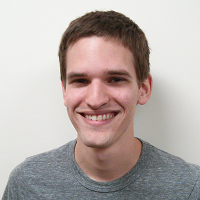
\includegraphics[width=\linewidth]{Grant}
\vspace{-22pt}
\end{wrapfigure}

\textbf{Grant Hernandez} is a senior at the University of Central Florida. He will be
graduating with a Bachelor of Science in Computer Engineering this summer. In
his spare time, Grant writes lots of code, reverse engineers binaries, plays in cyber
Capture the Flag competitions, dabbles in computer graphics, and tinkers with
embedded systems. He will be attending the University of Florida in fall 2015
to begin his Ph.D in Computer Engineering with a security research lab.

\vspace{0.5cm}
\begin{wrapfigure}{l}{0.4\linewidth}
\vspace{-12pt}
\centering

\includegraphics[width=\linewidth]{Jimmy}
\vspace{-22pt}
\end{wrapfigure}

\textbf{Jimmy Campbell} is a senior at the University of Central Florida. He will be
receiving a Bachelor of Science in Computer Engineering in August 2015. His
interests include embedded programming, mobile development, and web back-end
development. Jimmy will be taking a full time position with Microsoft as a
Software Development Engineer after graduating.

\vspace{0.5cm}
\begin{wrapfigure}{l}{0.4\linewidth}
\vspace{-12pt}
\centering

\includegraphics[width=\linewidth]{Joseph}
\vspace{-22pt}
\end{wrapfigure}

\textbf{Joseph Love} is currently a senior at the University of Central Florida and will
receive his Bachelor of Science in Electrical Engineering in August of 2015. He
is currently working with Direct Beam Incorporated and plans to pursue his
masters in Electrical Engineering during the Fall of 2015 at UCF with a focus
in Electromagnetics.
\end{document}
